
\documentclass[11pt]{article}
\usepackage{amsmath}
\usepackage{siunitx}
\usepackage{graphicx, float}
\usepackage[plain]{algorithm}

\topmargin=-0.45in
\evensidemargin=0in
\oddsidemargin=0in
\textwidth=6.5in
\textheight=9.0in
\headsep=0.25in


\title{Group Design Project: Consolidated Logbook}
\author{Alex Booth}

\bibliographystyle{plain}



\begin{document}
    \maketitle
    \newpage

    \section{Meeting Dates}
        \begin{enumerate}
            \item 14/02/2021
            \item 25/02/2021
            \item 04/03/2021
            \item 07/03/2021
            \item 10/03/2021
            \item 29/04/2021
        \end{enumerate}
        \hrule
    
    \section{Meeting 1 Notes}
        \begin{figure}[H]
            \centering
            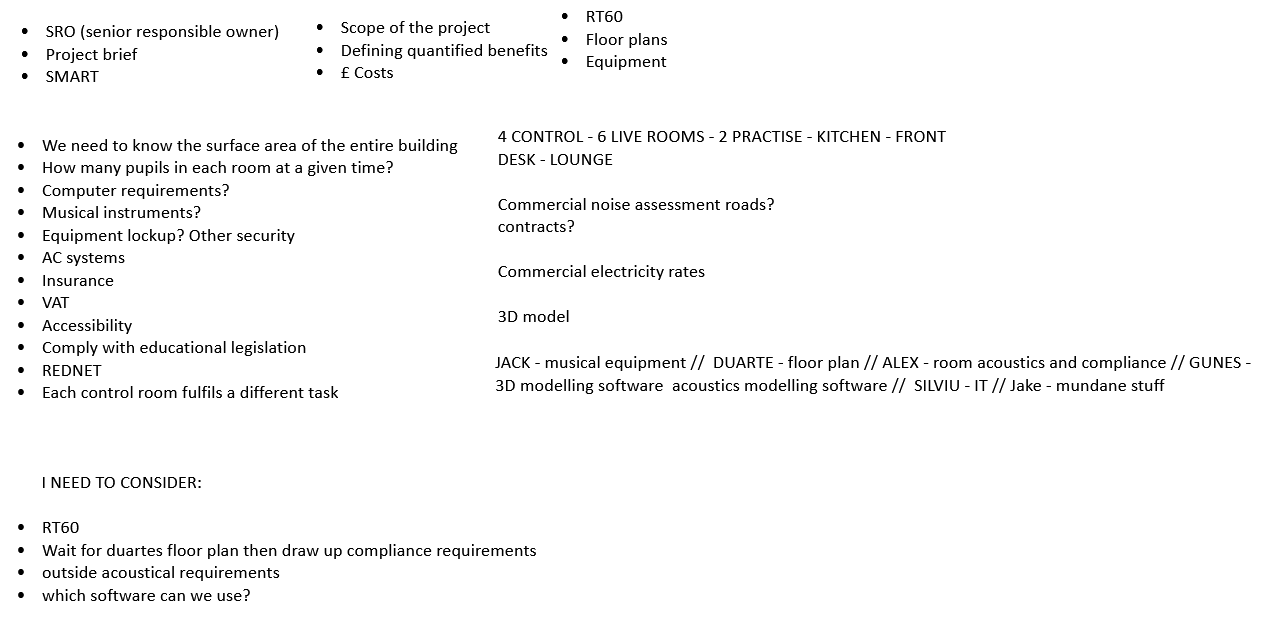
\includegraphics[scale=0.325]{resources/M1Notes.png}
        \end{figure}
        \hrule
        \vspace{0.5cm}
    \section{Meeting 2 Notes}
        \begin{figure}[H]
            \centering
            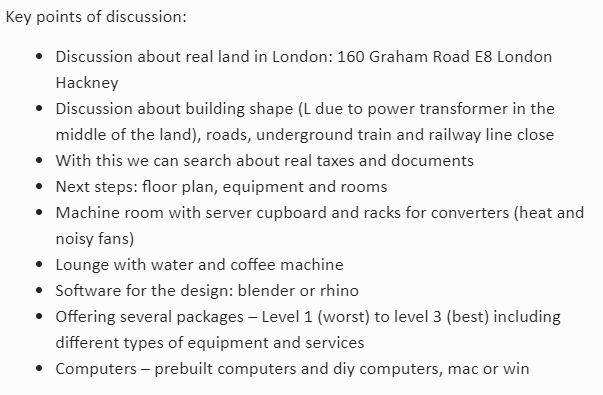
\includegraphics[scale=0.6]{resources/M2Notes.png}
        \end{figure}

    \section{Meeting 3 \& 4 Notes}
        \begin{figure}[H]
            \centering
            
\includegraphics[scale=1]{resources/lastMeets.png}
        \end{figure}
        \hrule
        \vspace{0.5cm}

    \section{Meetings 5 \& 6}
        Meetings 5  spent discussing final alterations to room acoustic treatment.
        Meeting 6 spent consolidating notes and beginning to plan formal report contents.  
    \section{My responsibilities and activities}
        \subsection{Week One}
            \begin{itemize}
                \item Reading and understanding the relevant legislation to the acoustic built environment in schools.
                \item Beginning to research industry methods of studio construction with room acoustics in mind.
                \item Discussed my delegated tasks with the group
                \item Began to develop an idea of the benefits of using a case study.
            \end{itemize}

        \subsection{Week Two}
            \begin{itemize}
                \item Presenting my findings from the previous week's research to my group.
                \item Presented and developed the idea of the 160 Graham Road case study to the group members not involved in the initial idea of the study.
                \item Investigated built environment acoustic modelling software solutions
            \end{itemize} 

        \subsection{Week Three}
            \begin{itemize}
                \item Making detailed notes on Lecture 3 and conducting further research - lec. 3 contained relevant information for my role
                \item Discarding the idea of using complex modelling software - most of mathematics needed for my work can be done as a series of algebraic equations and as such finite element analysis was not needed.
                \item Beginning to research methods of designing absorbers to target specific frequencies.
            \end{itemize}

        \subsection{Week Four}
            \begin{itemize}
                \item Analyzing the floor plan produced by another group member, and discussing tweaks to better fit acoustic criteria.
            \end{itemize}

        \subsection{Week Five}
            \begin{itemize}
                \item Preparing for presentation
                \item Making total absorption requirement calculations for each room.
            \end{itemize}

        \subsection{Week Six}
            \begin{itemize}
                \item Giving presentation
                \item Making notes and plans based on feedback
            \end{itemize} 
        \subsection{Week Six - Present}
            \begin{itemize}
            

\end{document}